\documentclass[]{article}
\usepackage{listings}
\usepackage{hyperref}
\usepackage{xcolor}
\usepackage{geometry}
\usepackage{csquotes}
\usepackage[]{setspace}
\usepackage[]{graphicx}
\usepackage[]{amsmath}
\usepackage[]{amsfonts}
\usepackage[]{hyperref}
\usepackage{caption}
\usepackage{subcaption}
\usepackage{graphicx}
\usepackage[
backend=biber,
style=authoryear-comp,
sorting=ynt]{biblatex}
\addbibresource{phdreflib.bib}

\geometry{margin=1in}
\setlength{\parskip}{6pt}
\setlength\parindent{0pt}
\setstretch{1}

%opening
\title{From Neural to Social Computation: Collective Intelligence in Networks of Complex Agents}
\author{Marie-Lou Laprise\footnote{Some of the ideas for this project were developed in collaboration with Kamesh Krishnamurthy (Princeton Physics \& PNI)}}

\begin{document}
	
	\maketitle
\section{Introduction}

\rightline{``\textit{Think how hard physics would be if particles could think}" --Murray Gell-Mann}

Social networks are not only emergent complex systems, like colonies of ants or neurons in the brain. They are also formed of complex, heterogeneous agents. This makes their dynamics particularly challenging to model, even in comparison to formidably complicated systems like the brain: this is not only one brain, but a large number of them, interacting with each other over time. 

Like other complex systems (including the humans that compose them), social networks map noisy inputs to useful outputs in a decentralized, emergent manner.  Through repeated interactions, social networks can collect and transmit information over a range of time scales, perform distributed computation,\footnote{ I loosely follow Crutchfield (\cite{crutchfieldCalculiEmergenceComputation1994}) by defining \textbf{computation} as a useful mapping from an input to an output; and \textbf{distributed} to mean that computation emerges from the time-varying state of a system of many interacting elements.} record social memories, and reproduce social institutions. A prominent example of this is exchange and price discovery in financial markets. In so doing, social networks can take a variety of forms, depending on the clustering of tightly connected agents, the presence of popular agents with exponentially more ties than others, and many other structural features.

The dynamics associated with structured networks of complex, heterogeneous agents, however, remain a blind spot for both social science and theories of collective computation. In studies of opinion formation, traditional models relied on linear dynamics that have limited expressivity and cannot replicate some frequently observed phenomena like the presence of threshold effects or the tendency of information to saturate. Meanwhile, in neuroscience or biophysics, rich and expressive nonlinear models of distributed computation have been developed and studied extensively. But they generally feature simple and homogeneous units; an adequate choice for modeling neurons or bacteria, but not social agents. 

\textbf{Research questions.} Can we extend nonlinear models of neural computation to explore how heterogeneous social agents collect and exchange noisy information to collectively form opinions and make decisions? How much heterogeneity and complexity can we add while keeping a tractable model that can be informative about social dynamics?

As a first step, in this project, I examine \textbf{how adaptive time constants change how networks of interacting agents break indecision in response to contradictory signals}, in order to form stable opinion patterns. I do so for three different types of network structure: random, scale-free, and small-world networks.

\textbf{RNN model of opinion formation.} In recent work, Naomi Leonard and colleagues developed a model of multi-agent opinion formation that takes a form similar to a recurrent neural network (RNN) (\cite{bizyaevaNonlinearOpinionDynamics2022}, \cite{leonardFastFlexibleMultiAgent2024}) (the “BFL” model; see Section 2.1). They introduced nonlinearity to model information saturation, in contrast to linear averaging models that dominated the field of opinion dynamics. The BFL model is able to break indecision in the face of contradictory inputs. It rapidly converges to a steady state of consensus (all agents agree) or disagreement (agreement within subgroups but not between them) in a way that, its authors argue, parallels the observed behavior of bees choosing a nesting site or voters choosing a candidate.

The BFL model features simple, homogeneous agents, without memory or intelligence. But in real social networks, agents dynamically adjust their reaction times, as they receive information from and about the social system of which they form part. Here, I take a first step towards richer agent-level behavior by adding an adaptive time constant (or gate) to the opinion update. I then examine the dynamics of the gated model for different signal strengths and different types of connectivity matrices, compared to the initial model, using simulations in Julia.

\section{Methods}
\subsection{The BFL model}

While the BFL model can model multi-opinion formation, here I focus on the case of two mutually exclusive opinions represented by a scalar value $z$. The agent favors a given option when $z>0$, he disfavors it when $z<0$, and he is neutral when $z = 0$.

Each agent is represented by coupled ODEs. Agents communicate through a connectivity network. The instantaneous rate of change of (1) the opinion $z$ of agent $i$ and (2) the susceptibility or excitability $u$ of agent $i$,\footnote{In the initial model, the $u$ term is called attention. Here, we call it susceptibility to avoid any confusion with other uses of the word attention in machine learning and neuroscience.} for a network of size $N$, are as follows:
\begin{align}
	\dot{z}_{i}(t) &= -d_{i}z_{i}(t) + S \left( u_i(t) \cdot  \sum^{N}_{j=1} J^z_{ij}z_{j}(t)  \right) + I_{i}(t) \\
	\tau^u \dot{u}_i(t) &= -u_i(t)+u_0+g^u \sum ^{N}_{j=1} J^u_{ij}(z_{j}(t))^2
\end{align}

\textbf{Differences with vanilla RNNs.} It should be emphasized at the outset that contrary to the traditional RNN case, each agent $i$ has access only to its own input $I_i$. The only way for an agent to access inputs that were distributed to other agents is indirectly, by communication through the adjacency graph. Contrary to RNNs in machine learning, parameters are not learned through back-propagation; they must be set as hyper-parameters (or could be learned locally). 

\textbf{Components of the opinion update.} In the opinion update, the first term corresponds to linear negative feedback or self-inhibition, the second term to nonlinear positive feedback or recurrent excitation, and the last term is a time-varying input $I_i(t)$ that includes external input (signal and noise) and internal bias.

\textbf{Role of susceptibility.} The susceptibility $u_i$ of an agent to network information controls the relative strength of the external input vs the recurrent excitation received from the network. The susceptibility update is independent of the input; it only depends on the strength of the opinions of connected agents received through the network. The intuition here is that you will pay more attention to the opinion of your friends if they are highly convinced than if they are neutral. If all your friends are neutral, you may ignore their input, and only use external information to make a decision. Conversely, if all your friends are highly convinced, you may use their opinion more than external information when making a decision.

\textbf{Other definitions.} The other terms are defined as follows. \begin{itemize}
	\item $d_{i} > 0$ is a damping or resistance coefficient. 
	\item $S: \mathbb{R} \rightarrow \mathbb{R}$ is a bounded, sufficiently smooth saturation function such that: $S(0)=0$; $S'(0)=1$; $S'''(0)\neq0$, which is set to be $tanh(x)$.
	\item $J^z \in \mathbb{R}^{N \times N}$ is the communication matrix and $J^u \in \mathbb{R}^{N \times N}$ is the susceptibility matrix (they can be the same or different).
	\item $u_0$ is a basal level of susceptibility and $g^u \geq 0$ is a susceptibility gain. Both are constant and homogeneous.
\end{itemize}

\textbf{Dynamical features.} \textit{Breaking indecision.} The system described by the BFL model is able to collectively break indecision when faced with contradictory inputs of equal strength. Indecision-breaking takes the form of an opinion cascade. This happens through \textbf{indecision-breaking bifurcations}, in which the system transitions to a multi-stable regime. The dynamic susceptibility state acts a bifurcation parameter for the transition. This is because the susceptibility state vector determines the relative importance, for each agent, of self-inhibition versus recurrent excitation from the network (including self-excitation).

\textit{From neutral to opinionated.} With neutral initial opinions and in the absence of inputs, the state vector representing the opinions of all agents remains at the zero fixed point, the only stable state. When some agents receive brief external inputs, the system may go back to the zero fixed point, or undergo an indecision-breaking bifurcation toward a regime of multi-stability, in which case the agents will converge to some stable opinionated state that will outlast the external inputs. Figure \ref{fig:replication} shows this opinion cascade appearing as inputs grow large, both in the original paper and as replicated for this project.

\begin{figure}
	\centering
	\begin{subfigure}[t]{0.8\textwidth}
		\centering
		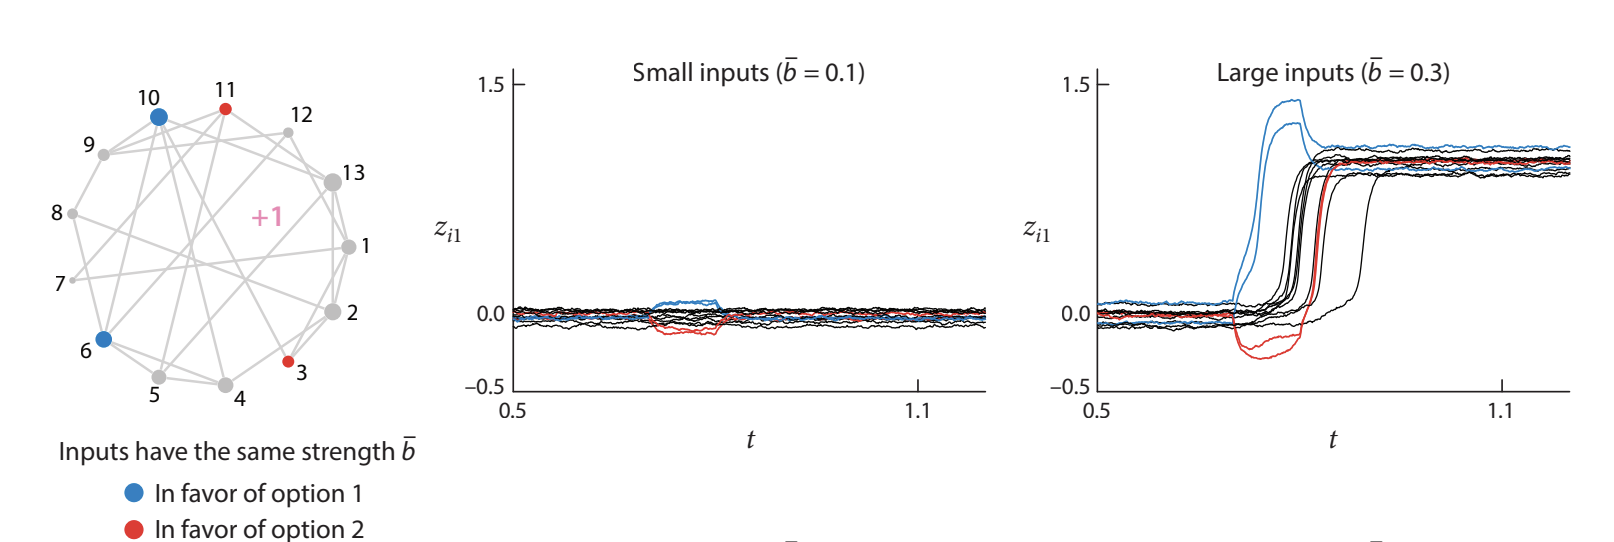
\includegraphics[width=\textwidth]{../plots/leonardfig2panA.png} 
		\caption{Results (Figure 2) of Leonard et al. 2024} \label{fig:damping1}
	\end{subfigure}
	
	\begin{subfigure}[t]{0.6\textwidth}
		\centering
		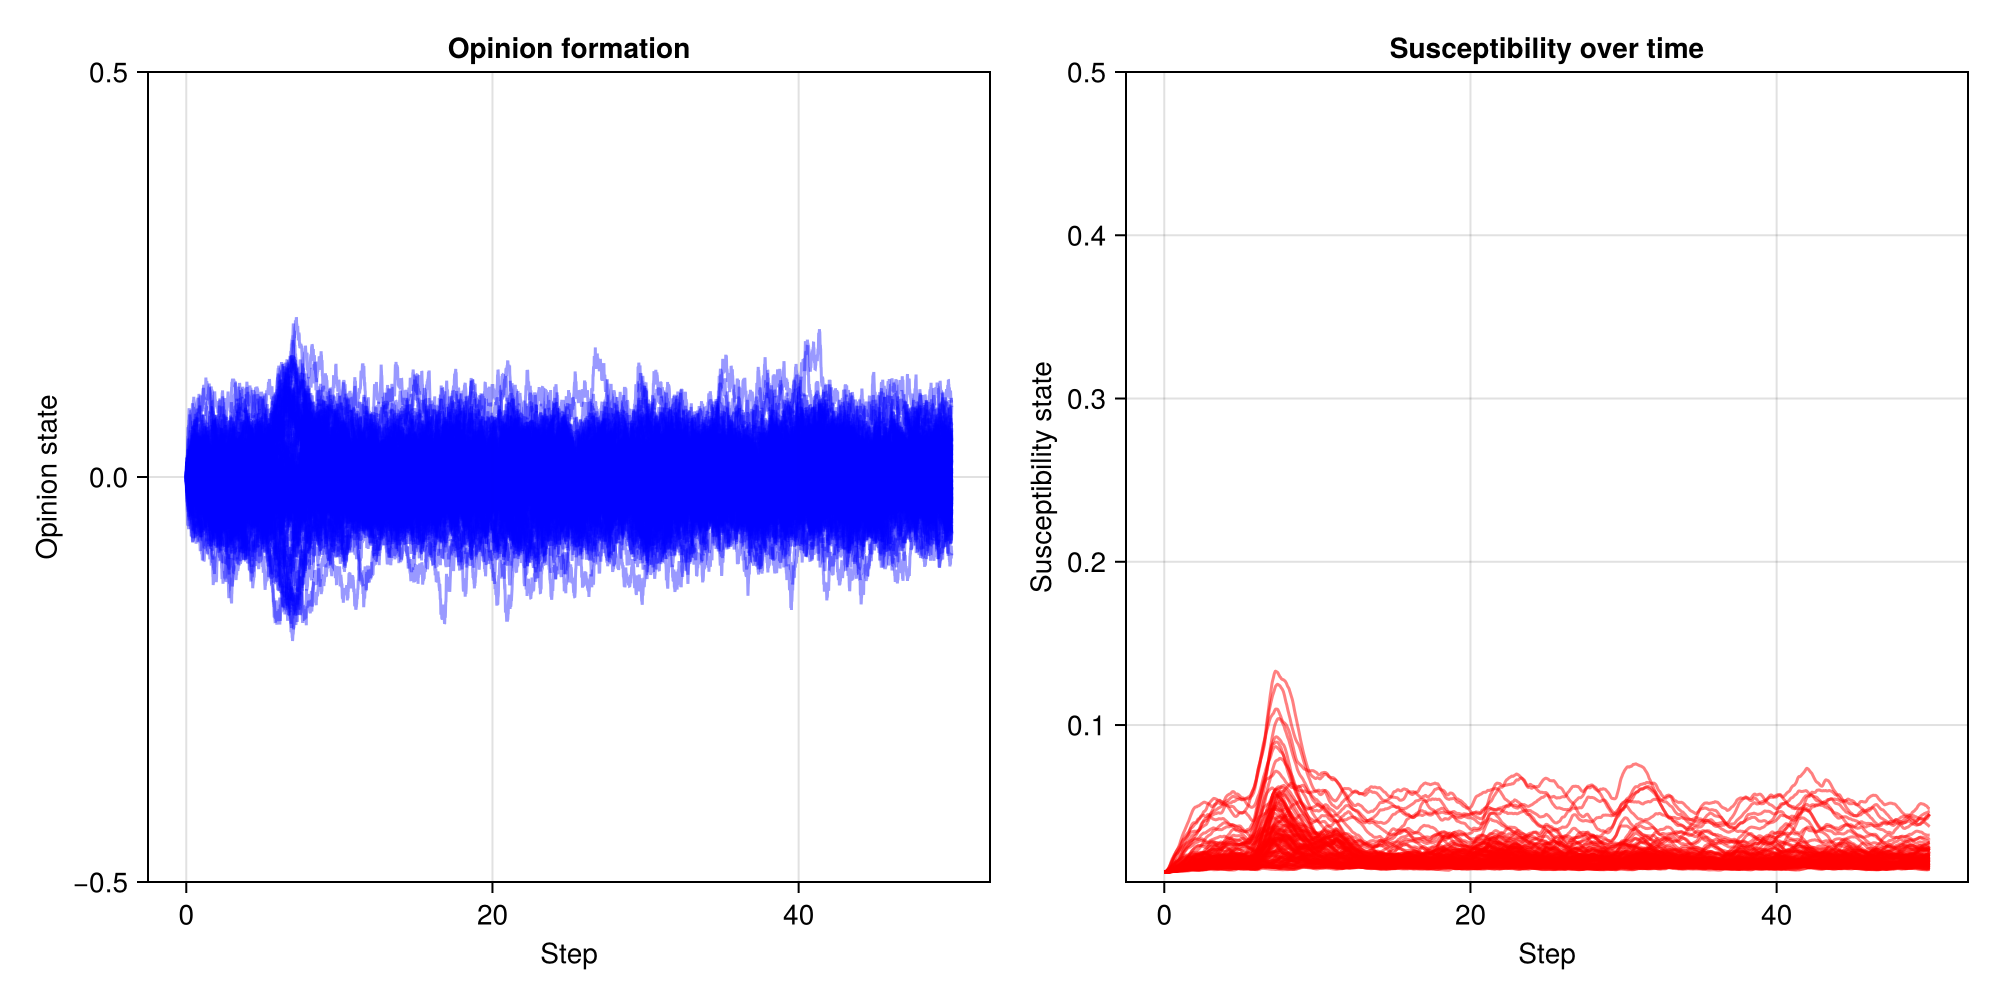
\includegraphics[width=\textwidth]{../plots/old/nog_constd_lowsig.png} 
		\caption{My simulation, input $b = \pm 0.1 $} \label{fig:damping2}
	\end{subfigure}
	
	\begin{subfigure}[t]{0.6\textwidth}
		\centering
		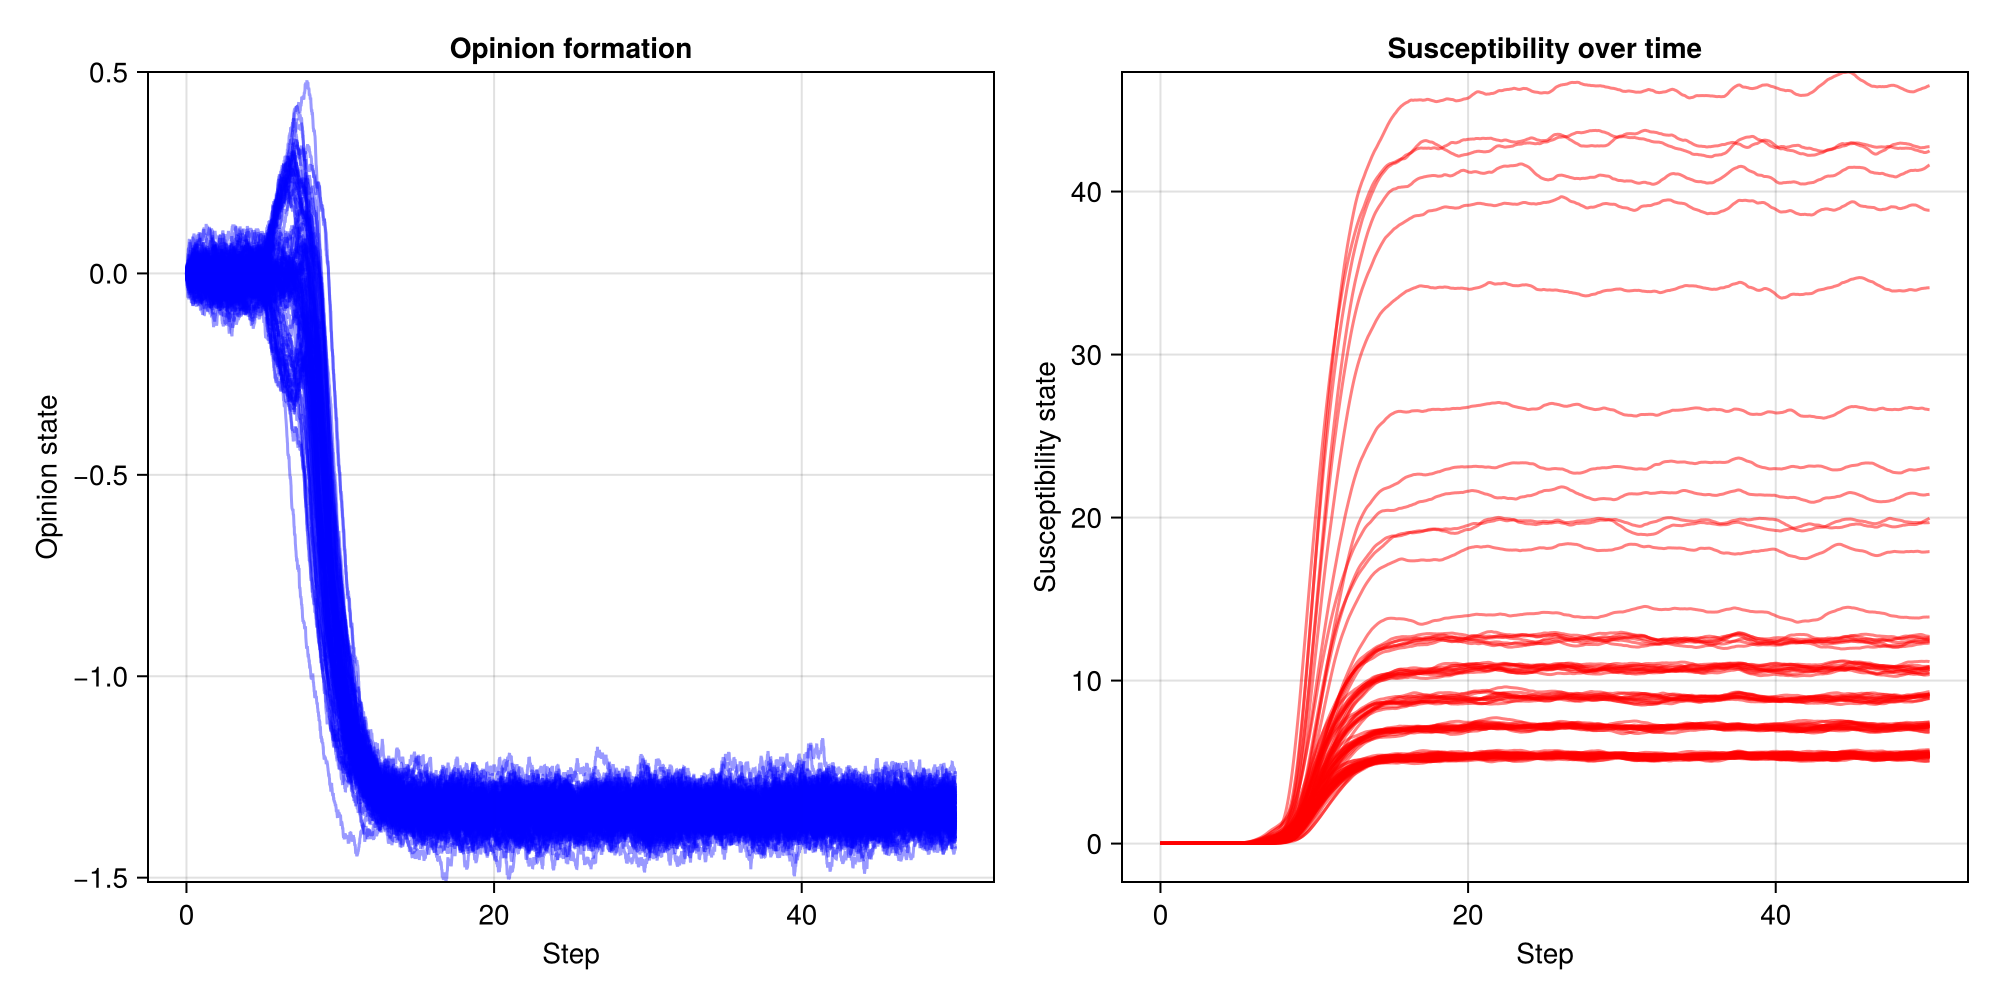
\includegraphics[width=\textwidth]{../plots/old/nog_constd_medsig.png} 
		\caption{My simulation, input $b = \pm 0.25 $} \label{fig:damping3}
	\end{subfigure}
	
	\caption{Opinion cascades under homogeneous damping and Gaussian noise, as external inputs grow larger. (\subref{fig:damping1}) is the top panel of Figure 2 of the BFL 2024 paper. In a small network of 13 agents, two agents receive a short signal of strength $b$ in favor of option 1 and concurrently, two agents receive a short signal of strength $-b$ in disfavor of option 1. Susceptibility state is not included. (\subref{fig:damping2}) and (\subref{fig:damping3}) are my simulations reproducing the same phenomena, with a network of 100 agents, with $d_i=d=0.75$. Opinion state in blue, susceptibility state in red. 25 agents receive a short signal in favor of option 1; 25 others receive a similar signal in disfavor. }\label{fig:replication}
\end{figure}

\textit{Sensitivity and robustness.} The authors also showed that at the bifurcation, indecision-breaking occurs rapidly, in a switch-like manner. As the system nears bifurcation, it becomes increasingly sensitive to certain inputs (in a selective manner). That is, it responds strongly to input vectors that align with the right eigenspace of the Jacobian at the bifurcation, but ignores input vectors that do not. Away from the bifurcation, opinion states remain stable even in the presence of small perturbations.

\textit{Stable disagreement.} The BFL model offered an elegant solution to a long-standing problem in the field of opinion formation: how to craft a system that may break indecision and generate stable disagreement as a function of inputs and initial conditions, rather than one that inevitably converges to consensus or avoids consensus only at the cost of a fixed, carefully hand-picked connectivity matrix (\cite{ravazziDynamicalSocialNetworks2021}, \cite{bernardoBoundedConfidenceOpinion2024}). This problem is sometimes called Abelson's diversity puzzle (\cite{abelsonMathematicalModelsDistribution1964}). 

\textbf{Assumptions of the BFL model.} A few things should be noted about the assumptions involved in this model.
\begin{enumerate}
	\item \textbf{Homogeneity.} Agents are homogeneous between each other (only their state distinguishes them) and across time (they do not learn or remember, only their state changes). For instance, agents all share a susceptibility time constant of $\tau^u$ and an opinion time constant of $1$. Agents all share an identical, non-parameterized input-output function. Agents all share a constant basal susceptibility and susceptibility gain. 
	\item \textbf{Balance of self-inhibition and recurrent excitation.} The self-inhibition implies that the opinion activation of each agent tends to revert to zero. This is balanced out by the self-excitation represented by the diagonal term of the $J^z$ matrix and the recurrent excitation represented by its non-diagonal terms, but modulated by the susceptibility state. At a low susceptibility, self-inhibition dominates and opinions tend to revert to zero. This is very close to the modeling of integrate-and-fire neurons.
	\item \textbf{Damping sets the opinion saturation levels.} While the damping coefficient $d_i$ is indexed as unit-specific, in most reported experiments, the original authors set a homogeneous value of $d_i=d$ for all agents. In the solution to the dynamical equations, $\pm d^{-1}$ becomes the scalar value of the stable opinionated states that the system may reach. That is, $d_i$ determines the value at which the opinion state of each agent $i$ will saturate. Diversity in $d_i$ would mean that instead of converging to identical scalar opinion states, agents would converge to opinion states of different magnitudes (agents are more or less convinced or extreme in their views). While this may seem realistic for social decision-making, this would be an artificial and hand-crafted way to achieve this result. Setting a homogeneous $d$ allows us to explore more interesting ways to achieve diversity. (As we will see in the results, gating may be one such way.)
	\item \textbf{Functional form and unboundedness of the susceptibility update.} It is not clear why the authors chose to square the opinion states in the susceptibility update. First, this assumes symmetry in the impact of negative and positive opinions, which is not obvious. I may not be equally affected by my friends being strongly in favor or in disfavor of something, although the difference between the two may be small enough that this does not impact results. In addition, because opinion states can grow larger than one (as determined by $d$ or the distribution of $d_i$) and the susceptibility update contains a sum of squared opinions, the susceptibility state can grow arbitrarily large.
\end{enumerate}

\subsection{Modified model}

\textbf{Adaptive time constants.} In real social networks, agents individually and dynamically adjust their reaction times, as they receive information from other agents and assess the state of the social system in which they are embedded. As a first step in modeling more complex agents, I add to the BFL model an adaptive time constant. In addition to better reflecting real social networks, the modified model should exhibit a richer dynamical range. Research on the physics of neural computation suggests that the nature of multiplicative interactions (or gating) in a model crucially determine its computational capabilities (\cite{krishnamurthyTheoryGatingRecurrent2022}). This change should allow the network to flexibly handle information on a range of time scales, and to enter regimes in which continuous attractors are formed. 

\textbf{Gated model.} I modify the model to include an input-dependent adaptive time-constant for the opinion update, in the form of a parameterized multiplicative gate that controls the rate of integration of the information received from the network (\cite{krishnamurthyTheoryGatingRecurrent2022}):

\begin{align}
	\dot{z}_{i}(t) &= \phi \left( x_i(t) \right) \cdot \left( -d_{i}z_{i}(t) + S \left( u_i(t) \cdot  \sum^{N}_{j=1} J^z_{ij}z_{j}(t)  \right) \right) + I_{i}(t) \\
	\tau^u \dot{u}_i(t) &=  -u_i(t)+u_0+g^u \sum ^{N}_{j=1} J^u_{ij}(z_{j}(t))^2 \\
	\tau^x \dot{x}_i(t) &= -x_i(t) +  \sum ^{N}_{j=1} J^x_{ij} S(z_j(t)) + k_i I_i(t)
\end{align}

\textbf{Definitions.} $J^x$ is a coupling matrix for the gate, $\phi (x) = (1 + e^{- \alpha x + \beta })^{-1}$ is a sigmoidal saturation parameterized by $\alpha$ and $\beta$, and $k_i I_i$ is a scaled version of $I_i$.

\subsection{Simulations}

\begin{figure}
	\begin{subfigure}{0.45\textwidth}
		\centering
		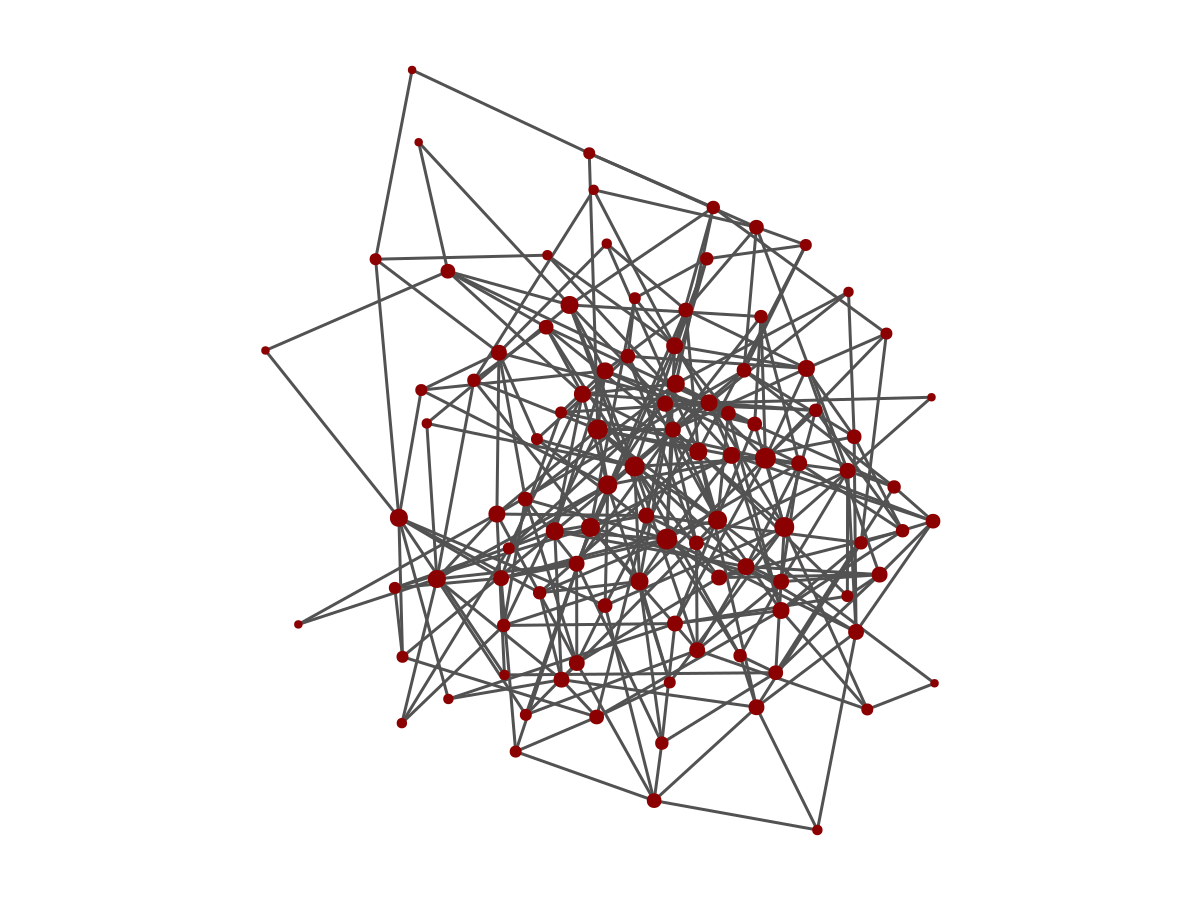
\includegraphics[width=0.8\linewidth]{../plots/g_erdosrenyi_n100_p3_s33} 
		\caption{ER graph}  \label{fig:subim11}
	\end{subfigure}
	\hspace{-1cm}
	\begin{subfigure}{0.45\textwidth}
		\centering
		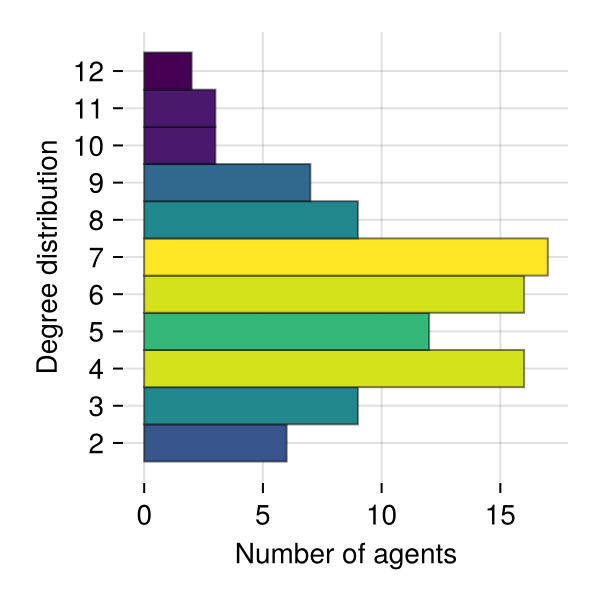
\includegraphics[width=0.5\linewidth]{../plots/g_erdosrenyi_hist_degree_n100_p3_s33}
		\caption{ER degree distribution} \label{fig:subim12}
	\end{subfigure}
	
	\begin{subfigure}{0.45\textwidth}
		\centering
		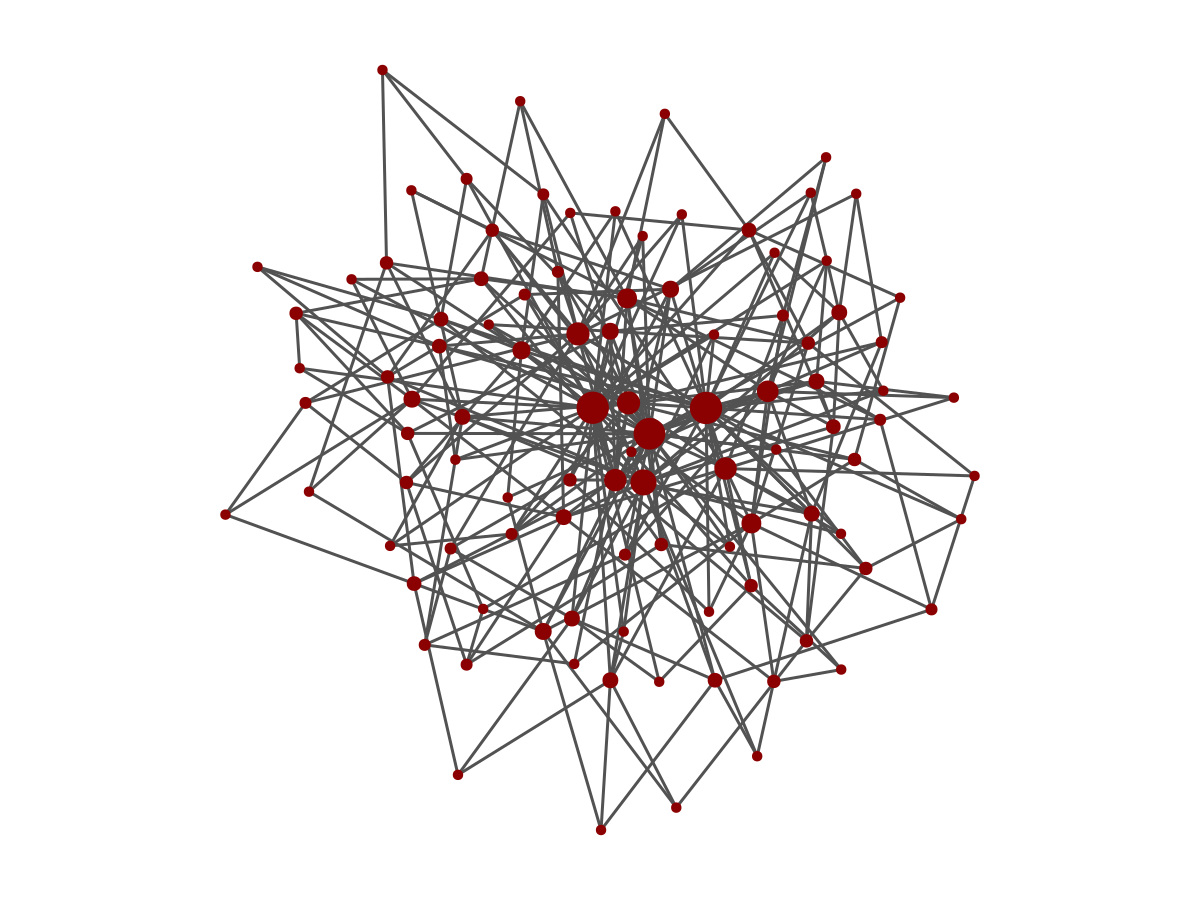
\includegraphics[width=0.8\linewidth]{../plots/g_barabasialbert_n100_m3_s33} 
		\caption{BA graph}  \label{fig:subim21}
	\end{subfigure}
	\hspace{-1cm}
	\begin{subfigure}{0.45\textwidth}
		\centering
		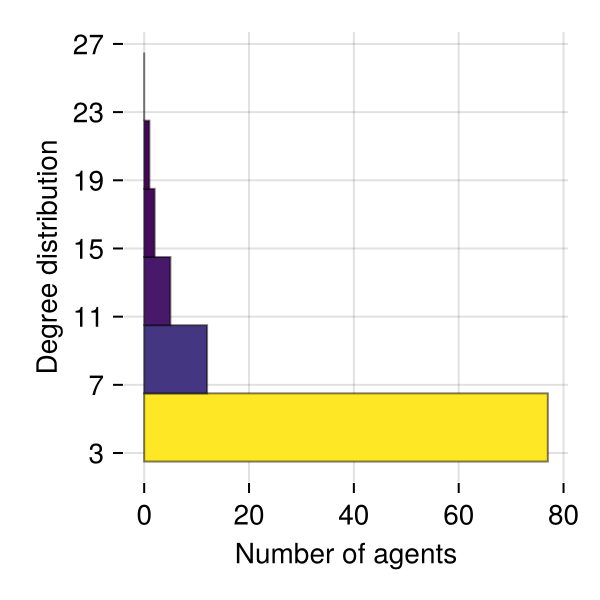
\includegraphics[width=0.5\linewidth]{../plots/g_barabasialbert_hist_degree_n100_m3_s33}
		\caption{BA degree distribution} \label{fig:subim22}
	\end{subfigure}
	
	\begin{subfigure}{0.45\textwidth}
		\centering
		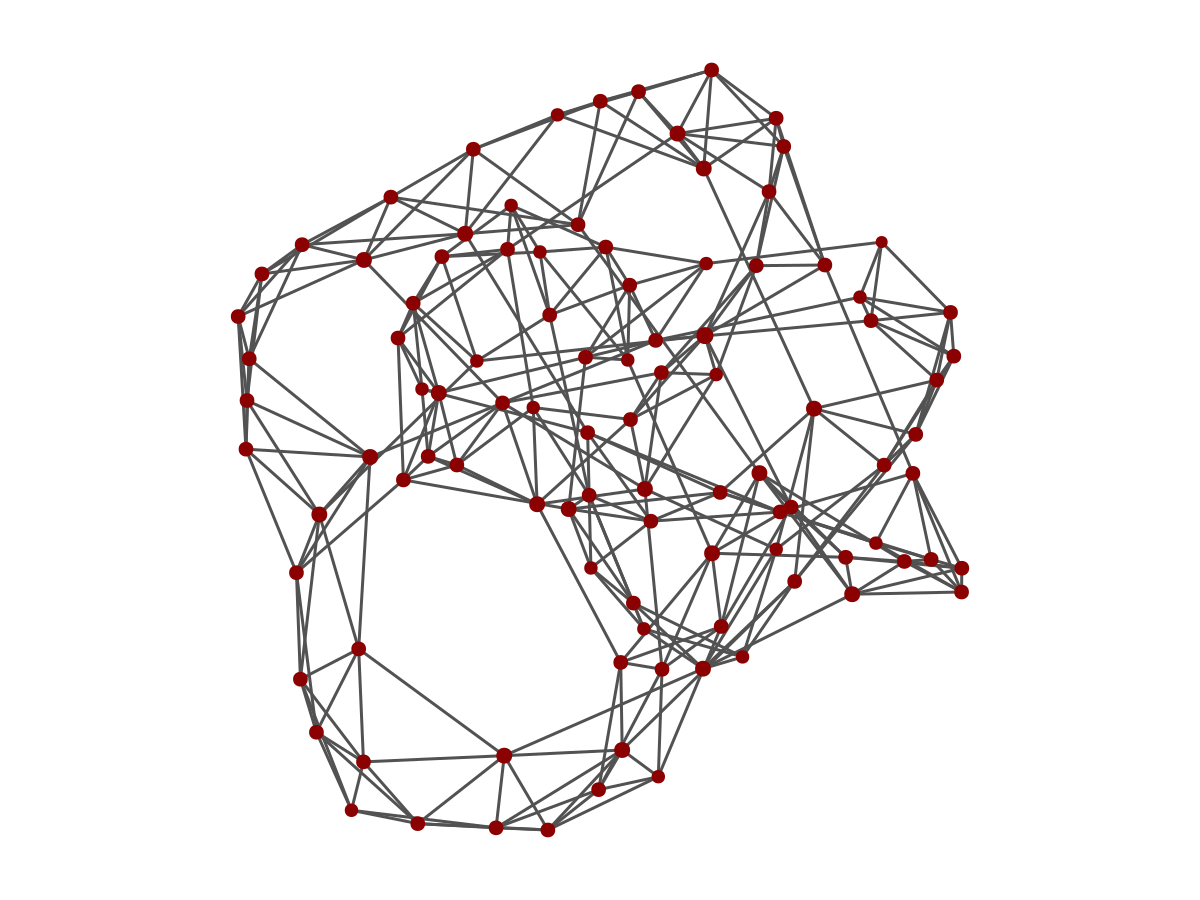
\includegraphics[width=0.8\linewidth]{../plots/g_wattsstrogatz_n100_k3_p01_s33} 
		\caption{WS graph}  \label{fig:subim31}
	\end{subfigure}
	\hspace{-1cm}
	\begin{subfigure}{0.45\textwidth}
		\centering
		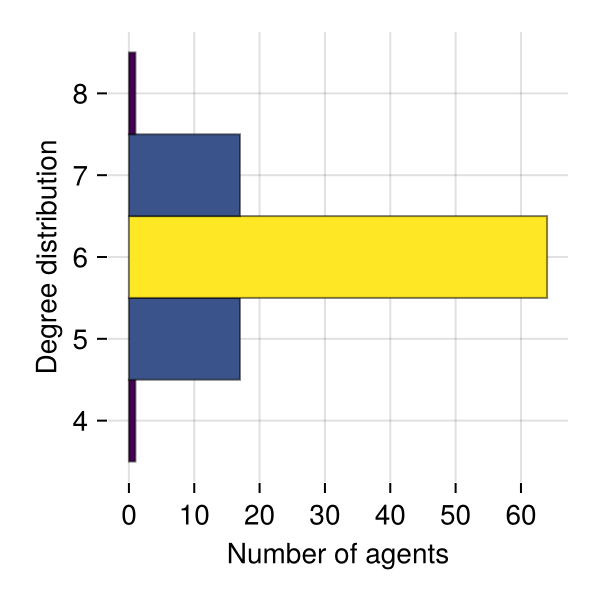
\includegraphics[width=0.5\linewidth]{../plots/g_wattsstrogatz_hist_degree_n100_k3_p01_s33}
		\caption{WS degree distribution} \label{fig:subim32}
	\end{subfigure}
	
	\caption{Example structure for 100 agents for the three types of social graphs explored in simulations.}
	\label{fig:graphtypes}
\end{figure}

In my simulations, I examined how gating impacts indecision-breaking bifurcations after the reception of contradictory signals of similar strengths. In all cases, one fourth of the agents receive a burst of positive signal, and another fourth concurrently receive a burst of negative signal. I compared the initial and gated models while varying the \textbf{strength of inputs} (low, medium, or high signal) and the \textbf{type of connectivity matrix} (random, scale-free, or small-world; see below). To more clearly visualize what happens in each combination of parameters, I turn off the noise in the system, so that evolution is deterministic based on the parameters and initial conditions.

For now, I simulated the system's evolution using the Julia \texttt{Agent.jl} package and Euler's approximation with a step size $h = 0.01$. I plan to replicate the results later using differential equations solvers and higher order approximations methods. All results are preliminary, as I have only had time to reproduce them with a couple of different seeds, and robustness across a variety of random seeds should be verified. Selected simulation results are included in a separate appendix. The code used to generate them is available at \href{http://github.com/m-laprise/socialcomputation}{github.com/m-laprise/socialcomputation}.

\textbf{Parameters for the simulations.} Some parameters must be held constant to focus on the effect of gating, signal strength, and connectivity. I set $N = 100$, which should be sufficient to generate graphs that are structurally distinct while remaining computationally tractable. After some exploration of the model's behavior in various regimes, I set the parameters as follows for all simulations in this report. $\tau^u = 1$, $g^u = 0.5$, $u_0=0$, $\tau^x = 5$, $\alpha = 2$, and $\beta = 0$. The damping coefficient is set constant at $d_i = d = 0.75$ and the scaling factor is sampled from a Gaussian, $k_i \sim \mathcal{N}(1,0.25)$, to create heterogeneity across agents. Any of these assumptions may be relaxed or modified in future work. 

\textbf{Initial conditions.} Agents are initialized at a random, almost neutral opinion state $z_i \sim \mathcal{N}(0, 0.01)$. Gating and susceptibility states are initialized at zero (if the basal susceptibility was above zero, we would initialize susceptibility at the basal level).

\textbf{Connectivity matrices $J^a$, $J^u$ and $J^x$.} For now, I set $J^a = J^u = J^x$, with the assumption that agents are both communicating with and paying attention to the same other agents (e.g. their friends). I also assume that $J^a$ is symmetric, which corresponds to the social graph being undirected, and its entries are zeros and ones (unweighted graph).

It might be particularly interesting to vary all these assumptions in future work. The first, for instance, to allow agents to have through the gating matrix some perception of the state of the broader social system in which they are embedded, and adjust their integration time accordingly. The second, to allow for unidirectional flow of information between agents, and the third, for heterogeneous flow.

I examine the dynamics associated with three different types of social graphs: Erdős-Rényi $G(n, M)$ (ER), Barabási-Albert (BA), and Watts-Strogatz (WS). I set the parameters of each of the three generators such that the average degree is comparable.\footnote{$N = 100$ agents. For ER, $M = N*3$ and $N*4$. For BA, $k = 3$ and $4$. For WS, $k = 6$ and $8$, $\beta = 0.1$.} ER is a classic random graph model without hubs or local clusters. BA is a scale-free network based on preferential attachment and has a power law degree distribution (and hence hubs). WS has a small-world structure and hence local clusters. While none is a perfectly realistic depiction of social networks, together they cover an interesting range of network structures.

Figure \ref{fig:graphtypes} illustrates this range by depicting a randomly generated graph of each type, along with its degree distribution.

\section{Results and discussion}

The dynamics of the model, with or without gating, are largely shaped by the structure of the connectivity matrix, with vastly different responses to external inputs depending if the social graph takes the form of an ER random network, a scale-free network, or a small-world network. 

The difference is illustrated in Figure \ref{fig:ng}, which shows indecision-breaking in response to contradictory inputs ($b = \pm 0.4$), in the absence of gating, on a randomly generated graph of each type. The behavior illustrated is consistent across a variety of random seeds: when presented with sufficiently strong contradictory inputs, ER random networks converge to a unique negative opinion value, scale-free networks to a unique positive opinion value, and small-world networks split into two groups of agents in stable disagreement with each other.\footnote{Different connectivity structures thus appear to exhibit bias in favor of positive or negative solutions, and this phenomena is robust to randomly generated networks and randomly distributed inputs with different random seeds.}

In all cases (without gating), the stable distribution of susceptibility states corresponds to the degree distribution of the underlying graph, as expected given the governing equations.

\begin{figure}
	\begin{subfigure}{\linewidth}
		\centering
		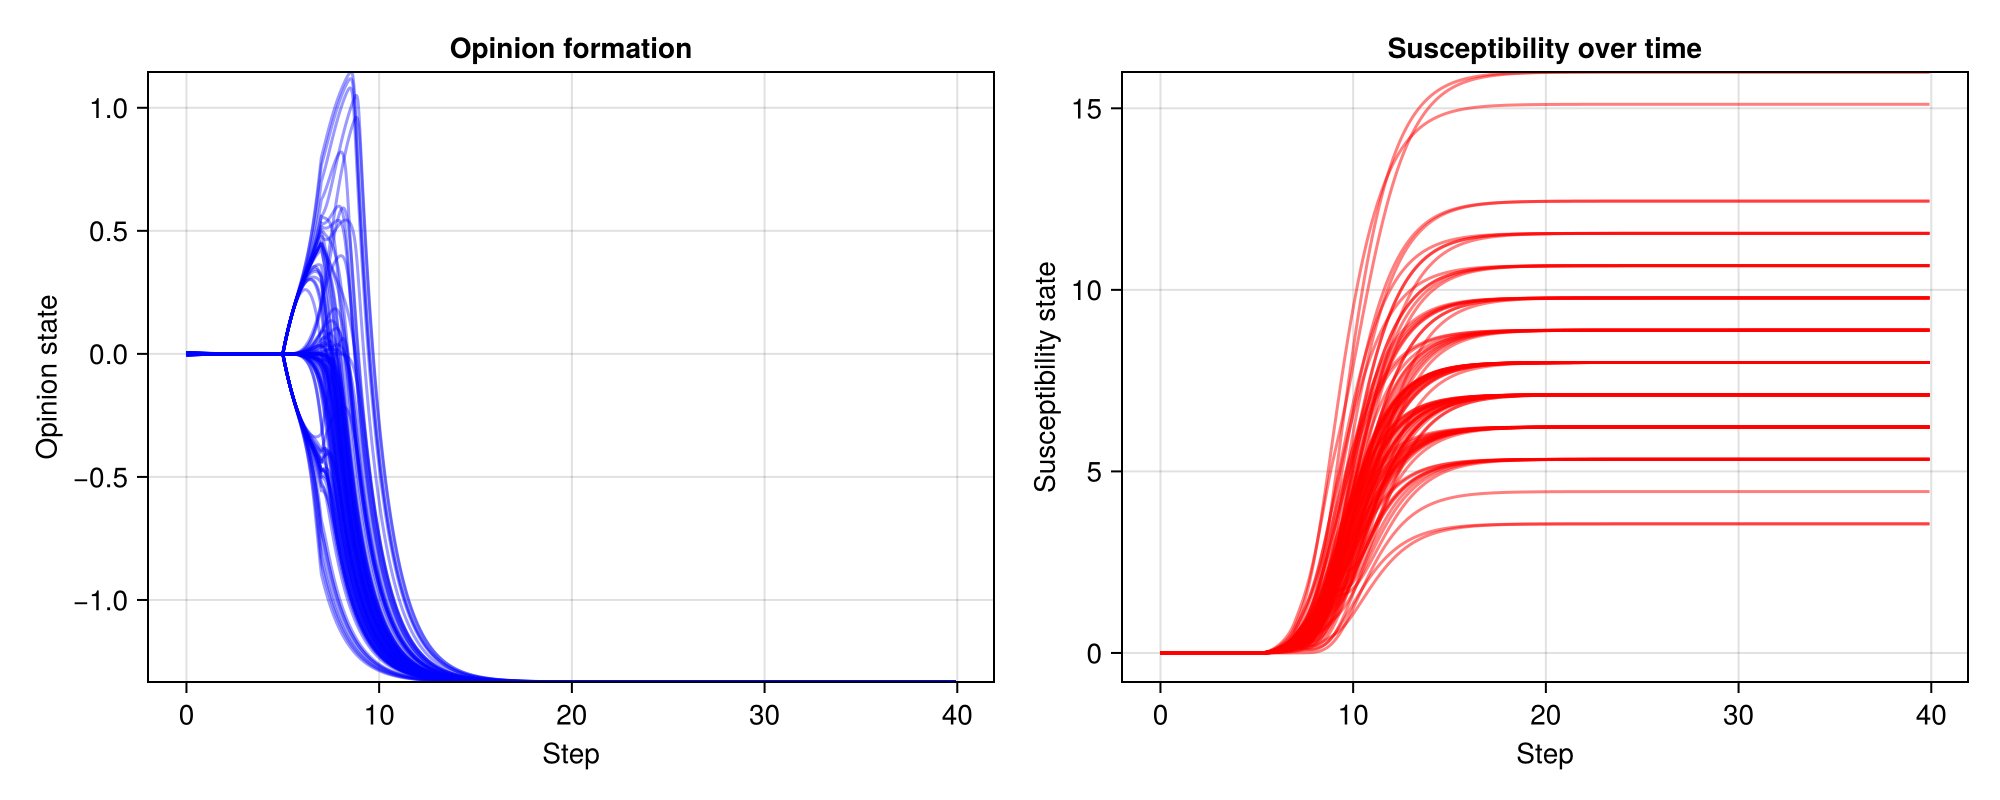
\includegraphics[width=0.75\textwidth]{../plots/nvar0_nog_homd_hisig_g05_ER4_s92391} 
		\caption{Erdos-Renyi random network}  \label{fig:ng1}
	\end{subfigure}
	
	\begin{subfigure}{\linewidth}
		\centering
		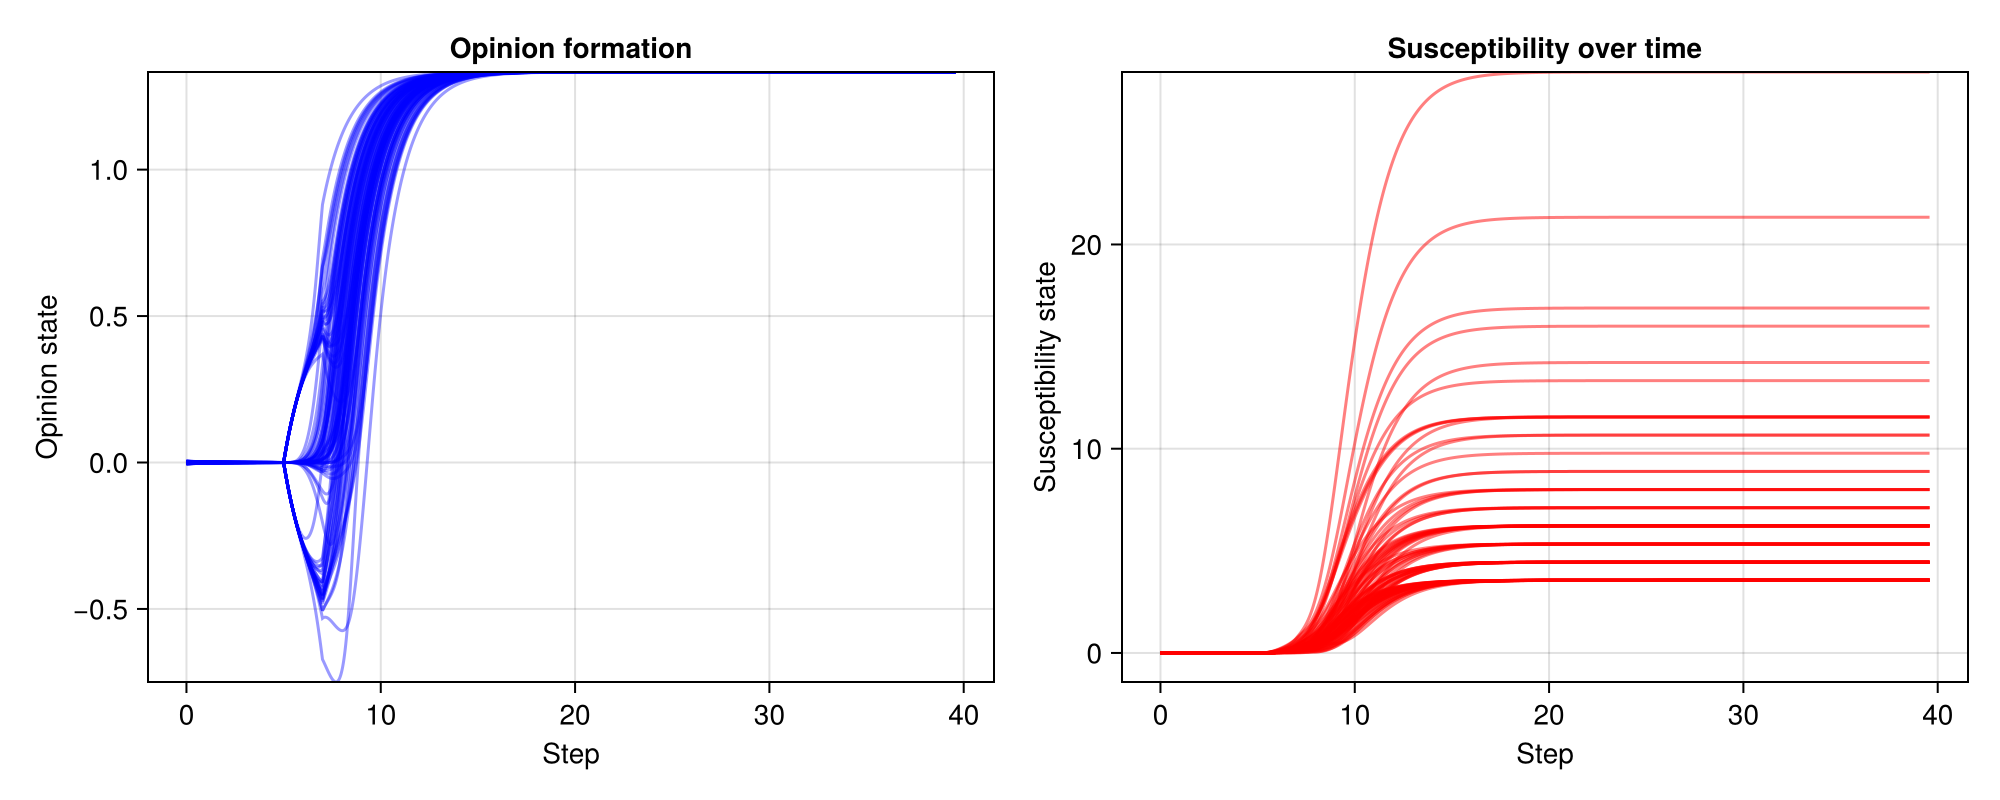
\includegraphics[width=0.75\textwidth]{../plots/nvar0_nog_homd_hisig_g05_BA3_s92391}
		\caption{Barabasi-Albert scale-free network} \label{fig:ng2}
	\end{subfigure}
	
	\begin{subfigure}{\linewidth}
		\centering
		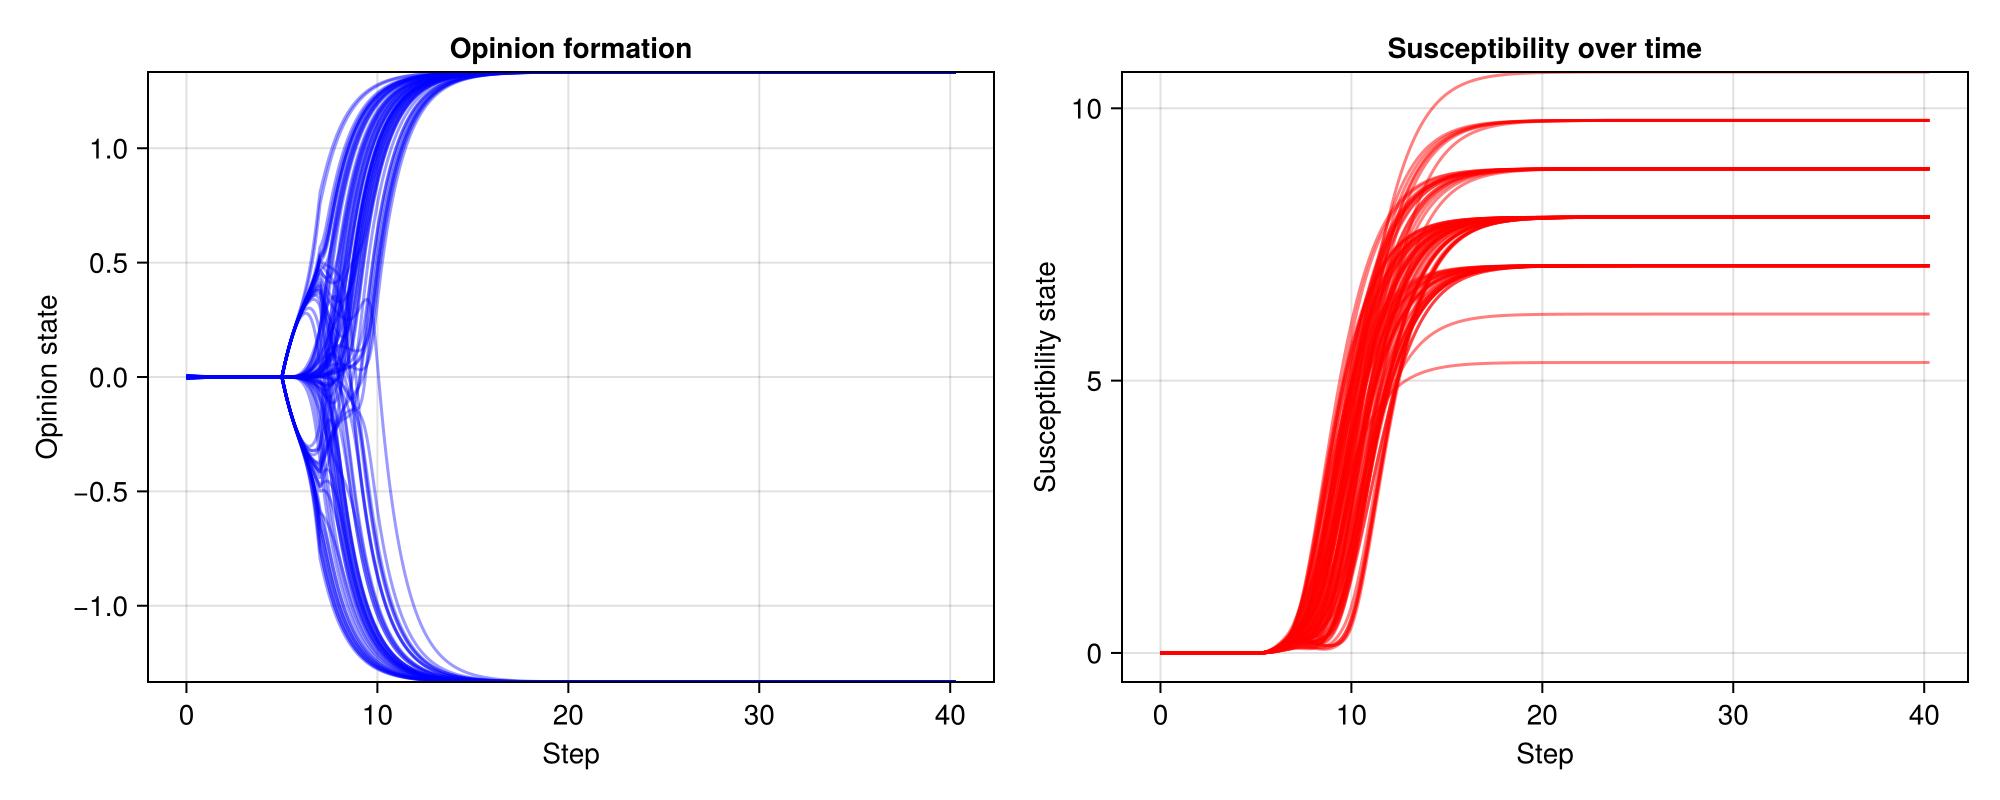
\includegraphics[width=0.75\textwidth]{../plots/nvar0_nog_homd_hisig_g05_WS4_s92391} 
		\caption{Small-world network}  \label{fig:ng3}
	\end{subfigure}
	
	\caption{Indecision breaking without gating, on three different types of social graphs.}
	\label{fig:ng}
\end{figure}

For scale-free networks, interestingly, as illustrated by Figure \ref{fig:ba}, gating makes very little difference to the dynamics. The opinion state evolution is almost unchanged, except that convergence is slightly slower. The susceptibility state evolution is unchanged and converges to the graph degree distribution, while the gating state also converges to the graph degree distribution. In contrast, for ER random and small-world networks, gating makes a large difference. I will examine each in turn.

\begin{figure}
	\centering
	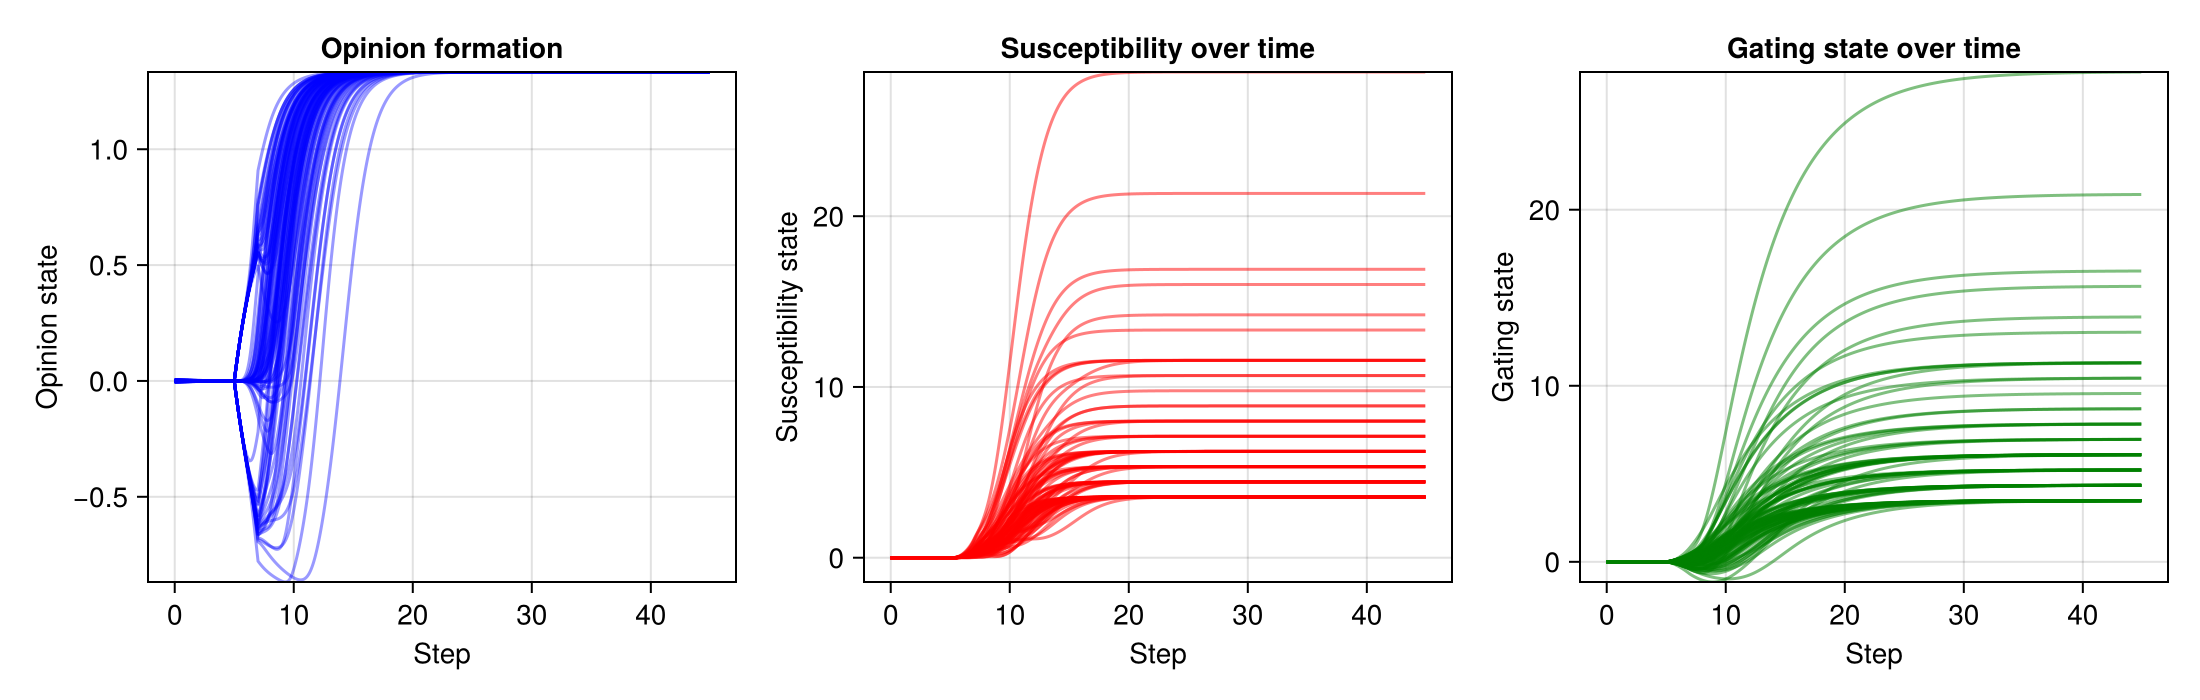
\includegraphics[width=0.75\linewidth]{../plots/nvar0_wg_homd_hisig_g05_BA3_a2_taux5_s92391}
	\caption{Same scale free network as \ref{fig:ng2}, with gating}
	\label{fig:ba}
\end{figure}

\textbf{Erdős-Rényi random network.} With an ER network as a connectivity graph, gating makes the dynamics of indecision-breaking more complicated and less homogeneous. 

Different behaviors are possible, depending on the exact structure of the graph, which varies with the random seed chosen. In social graphs for which agents converged to a unique negative opinion in the model without gating (Figure \ref{fig:er11}), with gating, they instead converge to a unique positive opinion, but they do so much slower, with agents switching over almost one by one, until consensus is achieved (Figure \ref{fig:er12}).

In some ER graphs, without gating, a medium signal strength is not sufficient to break indecision, and the system simply reverts back to the zero stable state (Figure \ref{fig:er21}). When adding gating to this network, however, indecision breaking does occurs, but in a new and interesting fashion. Most agents converge to a diversity of opinions in the same vicinity (rather than a unique scalar opinion), while a few agents converge to a unique opinion of the opposite sign (Figure \ref{fig:er22}).

Generally, across a variety of seeds, with gating, ER graphs often exhibit this convergence of agents to a diversity of opinions (instead of a single one), with or without a few contrarians holding the opposite view. This seems to be a more realistic representation of social decision-making, compared to the quick and uniform convergence to a single opinion seen in the initial model.

\begin{figure}
	\begin{subfigure}{\linewidth}
		\centering
		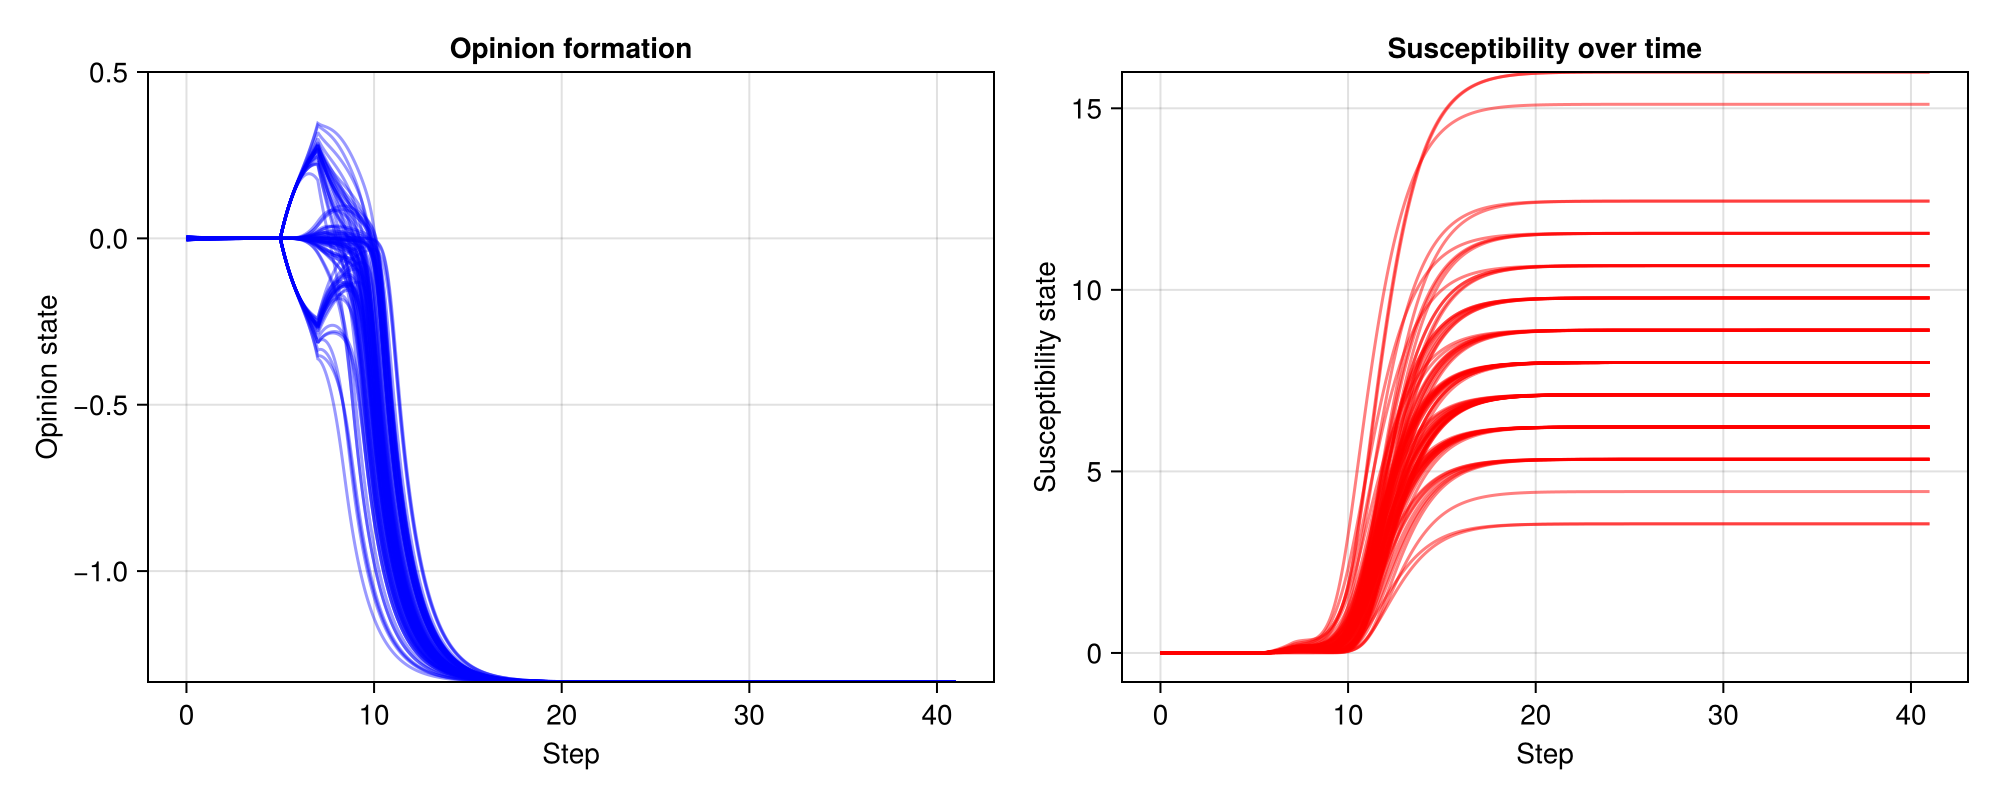
\includegraphics[width=0.55\textwidth]{../plots/nvar0_nog_homd_mediumsig_g05_er4_s92391_10000} 
		\caption{Medium signal ($b = 0.25$), without gating, variation 1}  \label{fig:er11}
	\end{subfigure}

	\begin{subfigure}{\linewidth}
		\centering
		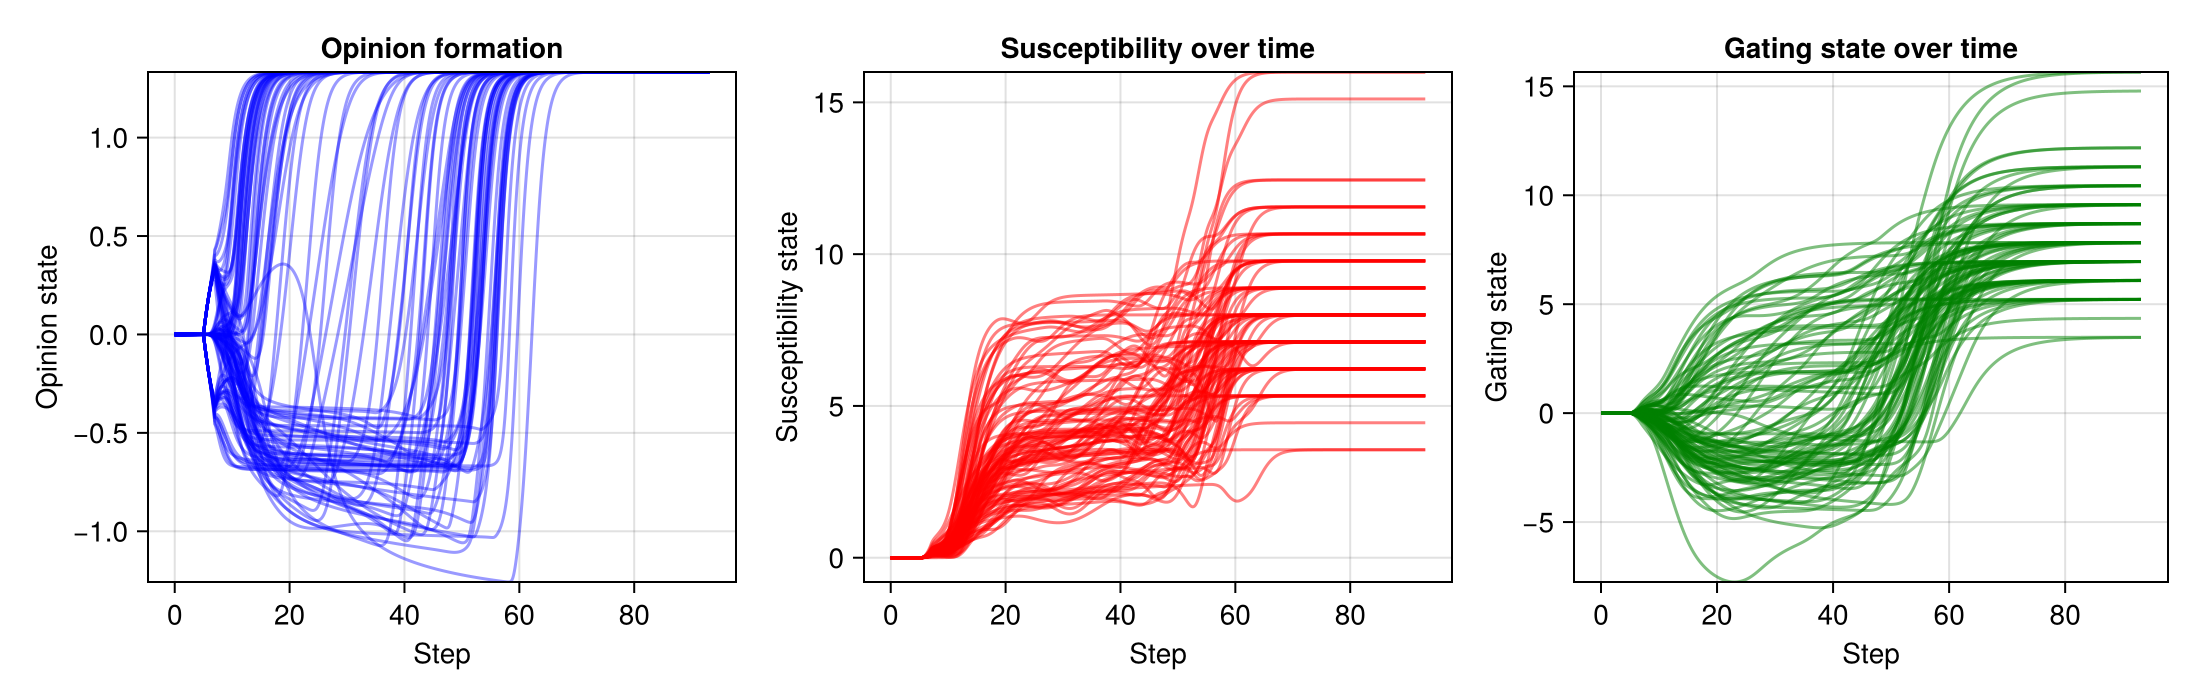
\includegraphics[width=0.75\textwidth]{../plots/nvar0_wg_homd_mediumsig_g05_er4_a2_taux5_s92391_10000}
		\caption{Medium signal ($b = 0.25$), with gating, variation 1} \label{fig:er12}
	\end{subfigure}
	
	\begin{subfigure}{\linewidth}
		\centering
		\includegraphics[width=0.55\textwidth]{../plots/nvar0_nog_homd_medsig_g05_er4_s2854} 
		\caption{Medium signal ($b = 0.25$), without gating, variation 2}  \label{fig:er21}
	\end{subfigure}

	\begin{subfigure}{\linewidth}
		\centering
		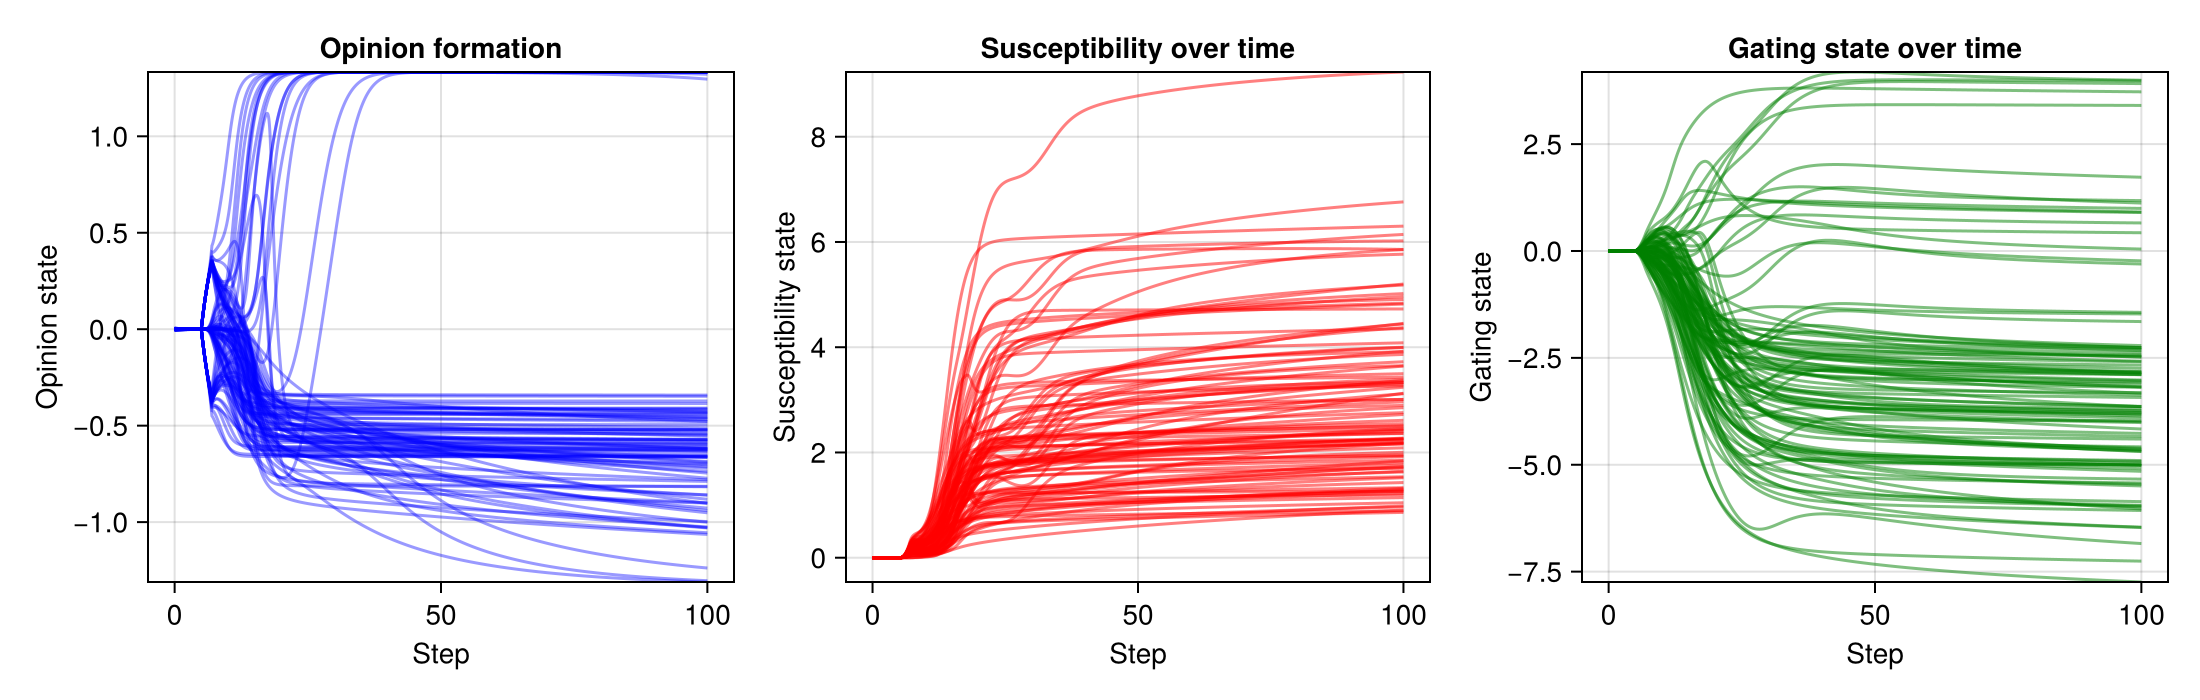
\includegraphics[width=0.75\textwidth]{../plots/nvar0_wg_homd_mediumsig_g05_er4_a2_taux5_s2854_10000}
		\caption{Medium signal ($b = 0.25$), with gating, variation 2} \label{fig:er22}
	\end{subfigure}
	\caption{Simulation results for ER random networks with different seeds. (a) and (b) are simulations on the same network, but without and with gating, respectively. The same goes with (c) and (d), on a different network.}
	\label{fig:ergraph}
\end{figure}

\textbf{Small-world networks.} Gating also completely transforms the dynamics of small-world networks. Without gating, the strength of the signal matters a lot to the dynamics, with the system undergoing a bifurcation from stable agreement (Figure \ref{fig:ws11}) to stable disagreement (Figure \ref{fig:ws21}) as the strength of the signal increases.

With gating, however, this bifurcation disappears, and the behavior becomes consistent for all signals strong enough to break indecision (Figure \ref{fig:ws21} and \ref{fig:ws22}). It seems that gating allows agents interacting in highly clustered networks to reach a state of agreement that they could not otherwise reach.

As was the case for some ER graphs, with gating, the system slowly converges to a positive scalar opinion. Here, about half the agents converge rapidly, and then, the others switch over one by one, hence the longer time to convergence.

\begin{figure}
	\begin{subfigure}{\linewidth}
		\centering
		\includegraphics[width=0.55\textwidth]{../plots/nvar0_nog_homd_medsig_g05_ws4_s92391} 
		\caption{Medium signal ($b = 0.25$), without gating}  \label{fig:ws11}
	\end{subfigure}
	
	\begin{subfigure}{\linewidth}
		\centering
		\includegraphics[width=0.75\textwidth]{../plots/nvar0_wg_homd_medsig_g05_ws4_a2_taux5_s92391}
		\caption{Medium signal ($b = 0.25$), with gating} \label{fig:ws12}
	\end{subfigure}
	
	\begin{subfigure}{\linewidth}
		\centering
		\includegraphics[width=0.55\textwidth]{../plots/nvar0_nog_homd_hisig_g05_ws4_s92391} 
		\caption{High signal ($b = 0.25$), without gating}  \label{fig:ws21}
	\end{subfigure}
	
	\begin{subfigure}{\linewidth}
		\centering
		\includegraphics[width=0.75\textwidth]{../plots/nvar0_wg_homd_hisig_g05_ws4_a2_taux5_s92391}
		\caption{High signal ($b = 0.25$), with gating} \label{fig:ws22}
	\end{subfigure}
	\caption{Simulation results for small-world networks. Without gating, stable disagreement occurs for sufficiently large input; otherwise, the agents converge.}
	\label{fig:wsgraph}
\end{figure}

\textbf{In summary}, for networks that are not scale free, gating makes the dynamics of indecision-breaking more complicated, less homogeneous, and potentially more realistic. In some cases, it slows down the dynamics, letting agents deliberate longer before settling in a steady opinion state. In other cases, it allows agents to settle into stable opinions that exhibit more variety, sometimes even with agents holding contrarian views. In more cases still, it allows indecision breaking in cases where that would not otherwise have occurred.

More work will be required to determine how gating effects those changes, how it interplays with noise, and why different graph structures interact with gating in such distinct ways, including why it has very little effect on scale-free networks. 

\newpage

\section{Future directions}

\textbf{Further modifications to the model.} As mentioned above, some changes to the form of the susceptibility update may be tested, to replace the squared opinion by a different function and add saturation so that the susceptibility state does not grow so large. In addition, it could be interesting to add some form of memory to the agents, or a more complicated input-output function.

\textbf{Further exploring the impact of various connectivity matrices.} In addition to more rigorously theorizing the link between the structure and density of the adjacency matrix and the dynamics of the system, future work should explore the impact of using weighted and directed connectivity matrices (to represent directed and heterogeneous flows of information), and the consequences of having different connectivity matrices associated with each of the state variables.

\textbf{Building predictive models of the environment from partial information.} Building predictive models of their environment is a crucial component collective intelligence. Here, I take model building to mean the discovery of structure and regularity in a dynamic environment so that a system can predict its next inputs better than at random (\cite{crutchfieldCalculiEmergenceComputation1994}). In social networks, the information acquired to do so is not only noisy, it is also partial and heterogeneous across agents. Ongoing research efforts (\cite{malachAutoRegressiveNextTokenPredictors2023}) suggest that in the machine learning setting, next-token prediction of structured sequences may enable a model to learn complex data-generating processes (DGP) accurately. However, if and how a DGP can be recovered by a network when different nodes each receive noisy and imperfect measurements of the sequences remains unknown. The BFL model only examines subjective beliefs, not the ability to converge to correct or useful answers. In the future, I plan to change the task from belief propagation to the collective recovery of a model of the environment from partial and heterogeneous information. This can be formalized as a hidden Markov problem. I will examine under what conditions the network is successful at recovering a ground truth from noisy, partial and asymmetric inputs. 

Interacting adaptive agents face some collective challenges that resemble those of neurons in the brain or nodes in an artificial network: (i) implementing distributed computation robustly and flexibly, over a range of time scales, and (ii) building predictive models of their environment. If there exists common principles underlying collective intelligence across settings, then models of neural computation may help us understand social computation. Conversely, models of social computation between complex agents might in turn suggest new models for how groups of neurons or regions of the brain interact to create a richer dynamical repertoire.

\printbibliography[heading=bibintoc, title={References}]

\end{document}